\begin{definition}
Une s\'erie temporelle est une suite chronologique de valeurs r\'eelles $x_t$ \`a des instants de temps r\'eguli\`erement espac\'es. 
% formule
\begin{equation}
(x_t)_{ t \in \Theta}
\end{equation}
avec $\Theta $ l'ensemble discret et fini des espaces de temps de dimension $n$.
\end{definition}
L'intervalle de temps entre deux mesures successives d\'epend de la s\'erie. 
Il peut s'agir d'une minute, d'une semaine, d'un jour, etc.
%G\'en\'eralement, les s\'eries temporelles s'utilisent dans les probl\`emes suivants :
G\'en\'eralement, les s\'eries temporelles sont utilis\'ees  pour comprendre les m\'ecanismes qui produisent ces observations. Ces m\'ecanismes sont associ\'es au temps et  permettent de faire les analyses suivantes :
\begin{itemize}
	\item La mod\'elisation : la repr\'esentation de la s\'erie sous la forme d'une fonction du temps.
	\item La pr\'evision : pr\'edire les donn\'ees futures \`a partir de valeurs pr\'ed\'ecentes.
	\item La d\'etection de rupture :  la s\'erie change-t-elle significativement \`a un instant $t$.
	\item La comparaison :  d\'eterminer la relation existante entre une s\'erie observ\'ee et d'autres s\'eries candidates.
\end{itemize}
Nous d\'ecrivons bri\`evement les mod\`eles d'analyses sur des s\'eries temporelles puis nous pr\'esentons l'objectif recherch\'e par l'analyse de ces s\'eries dans notre \'etude. 

\subsection{La mod\'elisation et la pr\'evison d'une s\'erie temporelle}
Un mod\`ele est une image simplifi\'ee de la r\'ealit\'e qui vise \`a traduire le fonctionnement d'un ph\'enom\`ene et permet de mieux les comprendre.
Nous distinguons deux types de mod\`eles :
\begin{itemize}
	\item Les mod\`eles d\'eterministes : ils utilisent les \'el\'ements de la statistique descriptive et suppose que l'observation de la s\'erie \`a la date $t$ est une fonction du temps $t$ et d'une variable $\epsilon_t$: 
	$$x_t = f(t, \epsilon_{t}).$$ 
	La variable $\epsilon_t$ est le r\'esidu ou l'erreur du mod\`ele et elle repr\'esente la diff\'erence entre la r\'ealit\'e et le mod\`ele propos\'e. 
	\newline
	Les deux mod\`eles les plus utilis\'es sont les suivants :
	\begin{itemize}
		\item Le mod\`ele additif : c'est la d\'ecomposition de la s\'erie en trois termes
			$$x_t = Z_t + S_t + Q_t $$ o\`u $Z_t$ est la tendance, $S_t$ la p\'eriodicit\'e et $Q_t$ les composantes (erreurs) identiquement distribu\'ees. $Z_t$, $S_t$ sont aussi d\'eterministes.
		\item Le mod\`ele multiplicatif : la variable $x_t$  est le produit de la tendance et d'une composante p\'eriodique :
		$$x_t = Z_t(1 + S_t)(1 + Q_t).$$
		Toutefois, l'application d'un logarithme nous permet de revenir au mod\`ele additif.
		$$y(t) = log(x_t) = log(Z_t) +log(1 + S_t) + log(1 + Q_t).$$
	\end{itemize}
	%L'utilisation de mod\`eles d\'eterministes pour la pr\'evision est \'el\'ementaire. Une fois d\'etermin\'ee la fonction $f$ \`a partir des donn\'ees observ\'ees $x_1 , ... , x_n$ , nous proposons une pr\'evision \`a la prochaine date par $\hat{X_{n+1}} = f(n+1)$.La pr\'ecision de cette pr\'evision peut aussi \^etre \'evalu\'ee par une estimation de la variance de $\epsilon_{n+1} = \hat{X_{n+1}} - f(n+1)$ . Cette estimation est r\'ealis\'ee par la variance empirique de la s\'erie des \'ecarts $\epsilon_i = X_{i} - f(i)$, consid\`er\'ee comme une s\'erie de variables al\'eatoires ind\'ependantes de m\^eme loi. La donn\'ee de cette variance empirique permettra de proposer un intervalle de confiance autour de la pr\'evision.

	\item Les mod\`eles stochastiques : ils font l'hypoth\`ese que les r\'esidus $\epsilon_t$ ne sont pas ind\'ependants et qu'il est possible de pr\'evoir les r\'esidus en partie. L'avantage r\'eside dans la r\'eduction de l'impr\'ecision de la pr\'evision des termes futurs de la s\'erie temporelle.  La variable $\epsilon_t$ devient une fonction des valeurs du pass\'e et d'un terme d'erreur $\eta_t$ $$\epsilon_t = (\epsilon_{t-1}, \epsilon_{t-2}, ... , \eta_{t}).$$
	Nous pouvons citer, comme exemple de mod\`eles couramment utilis\'es, les mod\`eles SARIMA, ARIMA et ARMA. Dans ces mod\`eles, la mod\'elisation porte sur la forme du processus $(\epsilon_t)$. Un exemple de mod\'elisation est le mod\`ele autor\'egressif lin\'eaire d'ordre $2$ avec des coefficients autor\'egressifs $a_1$, $a_2$ d\'efinis par 
	$$\epsilon_t = a_1 x_{t-1} + a_2 x_{t-2} + \eta_t,$$ o\`u $\eta_t$ est un bruit blanc.
\end{itemize}
Un exemple de s\'erie temporelle et de ses diff\'erentes composantes sont pr\'esent\'es dans la figure \ref{exempleSerieTemporelleComposante}. La s\'erie temporelle est la donn\'ee du trafic prise chaque mois des routes fran\c caises de $1989$ \`a $1996$.
La premi\`ere ligne est la r\'epresentation de la s\'erie temporelle et la seconde est celle de la tendance. Quant \`a la troisi\`eme  et la derni\`ere ligne, elles repr\'esentent respectivement la figure de p\'eriodicit\'e et les r\'esidus. La p\'eriode de la s\'erie est de $12$.
% ---- figure exemple de la serie temporelle et ses composante
\begin{figure}[htb!] 
\centering
\includegraphics[scale = 0.5]{exempleSerieTemporelleComposante.pdf}
%\includegraphics[scale = 0.5]{/home/willy/Downloads/exempleSerieTemporelleComposante.pdf}
\caption{ 
	D\'ecomposition de la s\'erie temporelle representant les valeurs mensuelles du trafic routier de l'autoroute $A7$ de $09/1989$ \`a $09/1996$. Repr\'esentation des composantes de la s\'erie temporelle.} 
\label{exempleSerieTemporelleComposante}
\end{figure}
%\FloatBarrier
% ---- figure exemple de la serie temporelle et ses composante

Les deux types de mod\`eles ci-dessus induisent des techniques de pr\'evision bien particuli\`eres. 
Sch\'ema--tiquement, ils s\'eparent la tendance de la saisonnalit\'e \'eventuelle. Puis ils cherchent \`a les mod\'eliser et \`a les estimer.  Enfin ils les \'eliminent de la s\'erie : ces deux op\'erations sont nomm\'ees
la {\em d\'etendancialisation} et la {\em d\'esaisonnalisation} de la s\'erie. Une fois ces composantes \'elimin\'ees, on obtient la s\'erie al\'eatoire $\epsilon_t$ :
%\vspace{-0.2cm}
\begin{itemize}
	\item Pour les mod\`eles d\'eterministes, cette s\'erie est consid\'er\'ee comme d\'ecorr\'el\'ee et il n'y a plus rien \`a faire.
	\item Pour les mod\`eles stochastiques, on obtient une s\'erie stationnaire (ce qui signifie que les observations successives de la s\'erie sont identiquement distribu\'ees mais pas n\'ecessairement ind\'ependantes) qu'il s'agit de mod\'eliser.
\end{itemize}
%L'utilit\'e de la mod\'elisation de s\'eries temporelles est couramment utilis\'e dans les 

\subsection{La d\'etection de rupture}
La d\'etection de rupture consiste \`a d\'eceler la pr\'esence d'un ou de plusieurs pics dans la s\'erie temporelle et \`a les localiser dans la s\'erie temporelle. 
D\'eterminer l'existence d'une rupture est d'autant plus difficile que cette derni\`ere n'est pas forc\'ement caract\'eris\'ee par un d\'ecalage de grande amplitude entre $x_t$ et $x_{t+1}$ par rapport \`a la dispersion des observations. 
Un enjeu de la d\'etection est donc d'\^etre sensible aux faibles variations tout en garantissant une certaine robustesse au bruit.
La th\`ese de master de {\em Flore Harl\'e} \cite{floreHarleDetectionRuptureMultiples2006} 
propose une m\'ethode de d\'etection de changements univari\'ee et multivari\'ee \`a la m\'ediane des segments, le segment \'etant une subdivision de la s\'erie temporelle. Les mod\`eles propos\'es sont exprim\'es par des fonctions de vraisemblance afin d'illustrer l'augmentation de la difficult\'e lors de l'ajout de nouvelles inconnues.

\subsection{La comparaison de  s\'eries temporelles}
Si deux s\'eries sont observ\'ees, nous pouvons nous demander quelle influence elles exercent l'une sur l'autre. 
Par exemple, \'etant donn\'ee deux s\'eries $X_t$ et $Y_t$, nous v\'erifions s'il existe par exemple des relations du type
$Y_t = a_1 \times X_{t+1} + a_3 \times X_{t+3}. $
\newline
Ici, deux questions se posent : tout d'abord, la question de la causalit\'e c'est-\`a-dire quelle variable (ici ($X_t$)) va expliquer l'autre (ici ($Y_t)$), ce qui conduit \`a la deuxi\`eme question, celle du d\'ecalage temporel: si une influence de $(X_t)$ sur $(Y_t)$ existe, avec quel d\'elai et pendant combien de temps la variable explicative $(X_t)$ influence-t-elle la variable expliqu\'ee $(Y_t)$ ?
\newline

%Dans notre cas d'\'etude, nous cherchons \`a comparer des s\'eries temporelles en supposant que les variation dans une s\'erie sont observables dans une autre s\'erie
%Ainsi, deux s\'eries $x_1$ et $x_2$ sont identiques s'il existe une s\'erie $k(t)$ de moyenne constante $K$ et d'\'ecart-type nul $\sigma_k = 0$ telle que 
%$$ \forall t \in \Theta, x_1(t) = k(t) \times x_2(t) .$$
Nous allons consid\'erer un r\'eseau de flots mod\'elis\'e par un graphe $G$ et les arcs portent des mesures. Les mesures sont mod\'elis\'ees par des s\'eries temporelles.
Dans notre cas d'\'etude, nous cherchons \`a comparer des s\'eries temporelles en supposant que les variations dans une s\'erie sont observables dans une autre s\'erie. Pour ce faire, nous rappelons que le coefficient de similarit\'e est une valeur indiquant la relation existante entre deux arcs et nous d\'efinissons la corr\'elation entre des arcs comme suit : 

\begin{definition}  Corr\'elation entre arcs\newline
Soit $corr$ le coefficient de similarit\'e entre les s\'eries $x$ et $y$ d\'efini de $\mathbb{R}^{n} \times \mathbb{R}^{n}
 \rightarrow [0,1]$ et 
 les arcs $A$ et $B$ contenant respectivement les s\'eries $x$ et $y$.
 \newline
Deux arcs $A$ et $B$ sont corr\'el\'es si et seulement si le coefficient de similarit\'e entre les s\'eries $x$ et $y$ est contenu dans $[0.5,1]$. 
($corr(x, y) \in [0.5,1]$)
\end{definition}
On dit alors que  $A$ et $B$ sont {\em fortement  corr\'el\'es} si 
le coefficient de similarit\'e est contenu dans l'intervalle $[0.7, 1]$ ($corr(x, y) \in [0.7,1]$) et {\em faiblement corr\'el\'es} si $corr(x, y)$ appartient \`a l'intervalle $[0.5,0.7[$ ($corr(x,y) \in [0.5, 0.7[$).
\newline

